\chapter{Solution}
\minitoc

The main goal of this solution is to develop a recommendation system for an e-commerce platform. 
In this context, users are referred to as customers or buyers ( representing individuals interacting with the platform which can be through a website or an app ), 
while products are referred to as items ( representing the goods offered for sale ).

To operate all the stages of the recommendation pipeline and the system components, 
a lot of infrastructure and DevOps work is required, from data ingestion to the deployment of the components.
The following sections will explain the system components and the deployment and technologies used in each stage of the recommendation pipeline.

The system components can be divided into the following categories:
\begin{itemize}
    \item API gateway
    \item Storage Components
    \item Recommendation Pipeline
    \item Caching Layer
    \item Automation and DevOps
\end{itemize}

\begin{figure}[H]
    \centering
    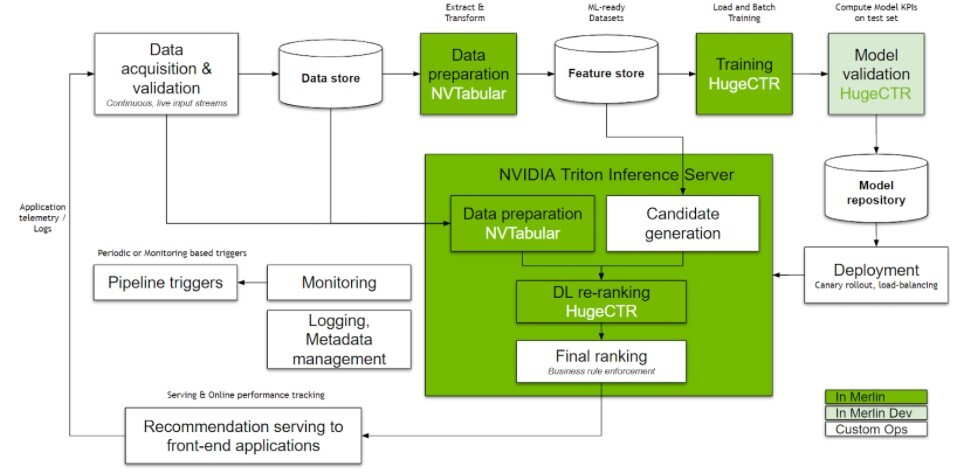
\includegraphics[width=1\textwidth]{assets/components.jpeg}
    \caption[System Components]{System Components \cite{NvidiaRecSysBestPractices}}
\end{figure}

Each component is explained in the following sections.

\section{API Gateway}

The API gateway, a RESTful API, is the entry point for the recommendation system.
It is responsible for handling all the requests and responses from the customers.
The main two functionalities of the API gateway are data ingestion and getting recommendations for a customer.

In addition to these functionalities, the API gateway is also responsible for authenticating and authorizing the requests.

\subsection{Data Ingestion Endpoints}

To handle the data ingestion, the API gateway exposes the following endpoints:
\begin{itemize}
    \item CRUD customers
    \item CRUD products
    \item Adding interactions between customers and products
\end{itemize}

Such endpoints interact mainly with the storage components to store the data.

\subsection{Recommendation Endpoints}

To get recommendations for a customer, the API gateway exposes the following endpoint:
\begin{itemize}
    \item Get recommendations for a customer
    \item Get similar products to a product
\end{itemize}

Those endpoints interact mainly with the recommendation pipeline and the caching layer to get the recommendations.

The first endpoint queries the caching layer to get the recommendations, and if the offline recommendations are not found in the caching layer, 
the API gateway queries the recommendation pipeline to get online recommendations, and then stores the recommendations in the caching layer, 
after getting the recommendations from the recommendation pipeline, 
the API gateway orders the recommendations using the output of the ranking stage and using business rules, then returns the top recommendations to the customer.

In the second endpoint, the API gateway queries the feature store to get the embeddings of the product and then executes an ANN search to get similar products.

\section{Storage Components}

The storage components are responsible for storing the data in different formats and stages, in addition to the models used in the recommendation system.
There are four main storage components in the system:

\begin{itemize}
    \item Main Database
    \begin{displayquote}
        The main database is an SQL database that stores the customers, products, and
         interactions data. In this project, a PostgreSQL \cite{Postgres} instance 
         deployed using AWS RDS \footnote{AWS Relational Database Service \cite{AwsRDS}}
         is used as the main database. 
         But in a bigger production environment, a distributed Data Warehouse such as 
         Amazon Redshift \cite{AwsRedshift} or Google BigQuery \cite{GoogleBigQuery} can be used.
    \end{displayquote}
    \item Online Feature Store
    \begin{displayquote}
        The feature store is a storage system that stores data in a format optimized for ML models. \cite{NvidiaFeatureStores}
        It also stores the embedding tables of the customers 
        and products, in addition to any other categorical features.
        This project uses FEAST \cite{feast} as the feature store, which supports using a Redis \cite{Redis} 
        cluster as an Online store, the Redis cluster is deployed using AWS ElastiCache \cite{AwsElastiCache}.
    \end{displayquote}

    \item Item Embedding Store
    \begin{displayquote}
        A vector database that stores the embeddings of the products
        while allowing them to be queried using an ANN search algorithm. 
        In this project, the item embedding store is a Redis \cite{Redis} cluster with the RediSearch \cite{RediSearch} module deployed using AWS ElastiCache \cite{AwsElastiCache}.
    \end{displayquote}

    \item Model Repository
    \begin{displayquote}
        After training the models, their parameters are stored in the model repository. In this project, the model repository is an AWS S3 bucket \cite{AwsS3}. 
    \end{displayquote}
    \item Results Store
    \begin{displayquote}
       To implement offline batch recommendations, the results of running the recommendation pipeline periodically for all users are stored in the results store. 
       In this project, the results store is a Redis cluster deployed using AWS ElastiCache \cite{AwsElastiCache}.
    \end{displayquote}
\end{itemize}

\section{Recommendation Pipeline}

The recommendation pipeline is the core of the recommendation system.
Deploying a recommendation pipeline requires an accelerated infrastructure optimized for deep learning and several MlOps workflows.

It starts with the candidate generation stage, where a set of thousands of candidate products for each customer is chosen among millions of products.
Then the filtering stage filters the candidate items according to business rules and constraints, the scoring stage ranks the candidate items and finally the ordering stage orders 
the scored items and selects the top items to be recommended to the customer.

\subsection{Candidate Generation (Retrieval)}

To generate the candidate items for each customer, the system starts by retrieving the embeddings of the customer and the products from FEAST (the feature store).

\subsubsection{Two Tower Model (Offline Retrieval)}

During training (offline), the system uses a two-tower model, where the customer and product embeddings are produced through two separate towers, 
and the output of the two towers is used to compute the similarity between the customer and the products.

The products' embeddings are stored in a vector database, which is the item embedding store.

The training of the two-tower model is done using a distributed training framework, in this case,
 it was done using Merlin HugeCTR \cite{NvidiaHugeCTR} deployed on AWS SageMaker \cite{AwsSageMaker} inside a Merlin HugeCTR container \cite{HugeCTRContainer}.

\subsubsection{ANN (Online Retrieval)}

During inference (online), using two separate towers to retrieve the candidate items for each customer is not efficient. \cite{NvidiaFeatureStores}
To reduce the latency of the responses, the system uses only the customer tower to generate the embeddings of the customers,
after that, an ANN search algorithm is used to retrieve the candidate products from the item embedding store.

In production, the user tower is deployed using Nvidia Triton Inference Server \cite{Triton} on 
AWS SageMaker \cite{AwsSageMaker} inside a Merlin Inference container \cite{NvidiaMerlinInference} from Nvidia's NGC \cite{NvidiaNGC}.

\subsection{Rule Based Filtering (Filtering)}

After retrieving the candidate products for each customer, the system filters the candidate products according to business rules and constraints.
In an e-commerce platform, the business rules and constraints usually include the availability of the products, the customer's location and shipping availability to it.


The filtering workflow is implemented using NVTabular \cite{MerlinNVTabular}, and the workflow is stored in the model repository.

In production, the filtering workflow is deployed with the deep learning ranking model in the same container.

\subsection{Deep Learning Ranking Model (Scoring)}

This stage is the core of the recommendation pipeline, where the system ranks the candidate and filtered products and selects the top products to be recommended to the customer.

To rank the products, a deep learning ranking model is trained using the historical data of the interactions between the customers and the products.
Each categorical feature is replaced with its embedding and those embeddings are stored in the feature store during offline training. 
After training the model, the model's parameters are stored in the model repository.

The model's output is the ranking score of each product for each customer, which is the probability of the customer interacting with the product.

The ranking model that was used in this project is the DLRM \cite{facebook_dlrm} proposed by Facebook.
% TODO: fix this
Instead of implementing the DLRM from scratch, 
the system uses Merlin Models \cite{MerlinModels}
 implementation of the DLRM, 
 which is optimized to run accelerated on Nvidia GPUs using the HugeCTR \cite{NvidiaHugeCTR} framework.

The DLRM is trained using a distributed training framework, in this case, it was done using Merlin HugeCTR \cite{NvidiaHugeCTR} deployed on AWS SageMaker \cite{AwsSageMaker} inside a Merlin HugeCTR container \cite{HugeCTRContainer} from Nvidia's NGC \cite{NvidiaNGC}.

In production, the DLRM is deployed using Nvidia Triton Inference Server \cite{Triton} on a Merlin Inference container \cite{NvidiaMerlinInference} from Nvidia's NGC \cite{NvidiaNGC}.
AWS SageMaker \cite{AwsSageMaker} automatically scales the number of instances of the Triton Inference Server based on the load.

\subsection{E-commerce ordering logic (Ordering)}

After getting the ranking score of each product for the customer, the system orders the products using the ranking score and business rules, 
then selects the top products to be recommended to the customer.


In the context of an e-commerce platform, the ordering logic includes promoting products (sponsored products), 
where the sponsored products are put on top of the list if they exceed a certain threshold score.

The following equation represents the final score of the product which is used to order the products:

\textbf{New score = { 1.0  if (IsPromoted AND RankingScore >= Threshold) else RankingScore }}

The ordering stage is implemented in the API gateway since the number of products to be ordered after the ranking is very small.


\section{Storing Results}

To enhance the performance of the recommendation system, the results of online recommendations are stored in an in-memory caching layer.
In addition to that, the results of running the recommendation pipeline periodically for all users are stored in the results store.

This is done to provide the recommendations with ultra-low latency and to provide the recommendations in case of a failure in the recommendation pipeline or overload.

\section{Automation and MlOps}

To keep the recommendation system running and to keep the models up to date, a lot of automation and DevOps work is required.
The main task that needs to be automated is the periodic training of the models and the deployment of the models and the workflows.

To run periodic tasks a cloud-native service similar to cron jobs is required, in this project, AWS Batch \cite{AwsBatch} was used.
AWS Batch allows running computing workloads on the cloud, in an automated and scalable way.

The job should respawn the training environment and run the training workflow, then store the model's parameters and the workflow in the model repository, in addition to storing the embeddings in the feature store.

